\section{DCF Driver and Terminal-Value Audit}

Growth, reinvestment, WACC and terminal closure are shared across gold engines. Table~\ref{tab:dcf_inputs} summarizes the corporate assumptions.

\subsection{Growth, ROIC and reinvestment}
Growth and ROIC converge linearly to their stable levels over five years. Reinvestment follows $b_t=g_t/ROIC_t$, linking growth to the capital required to sustain it (Figure~\ref{fig:dcf_driver_schedule}).

\noindent\begin{minipage}{\columnwidth}
{\centering
  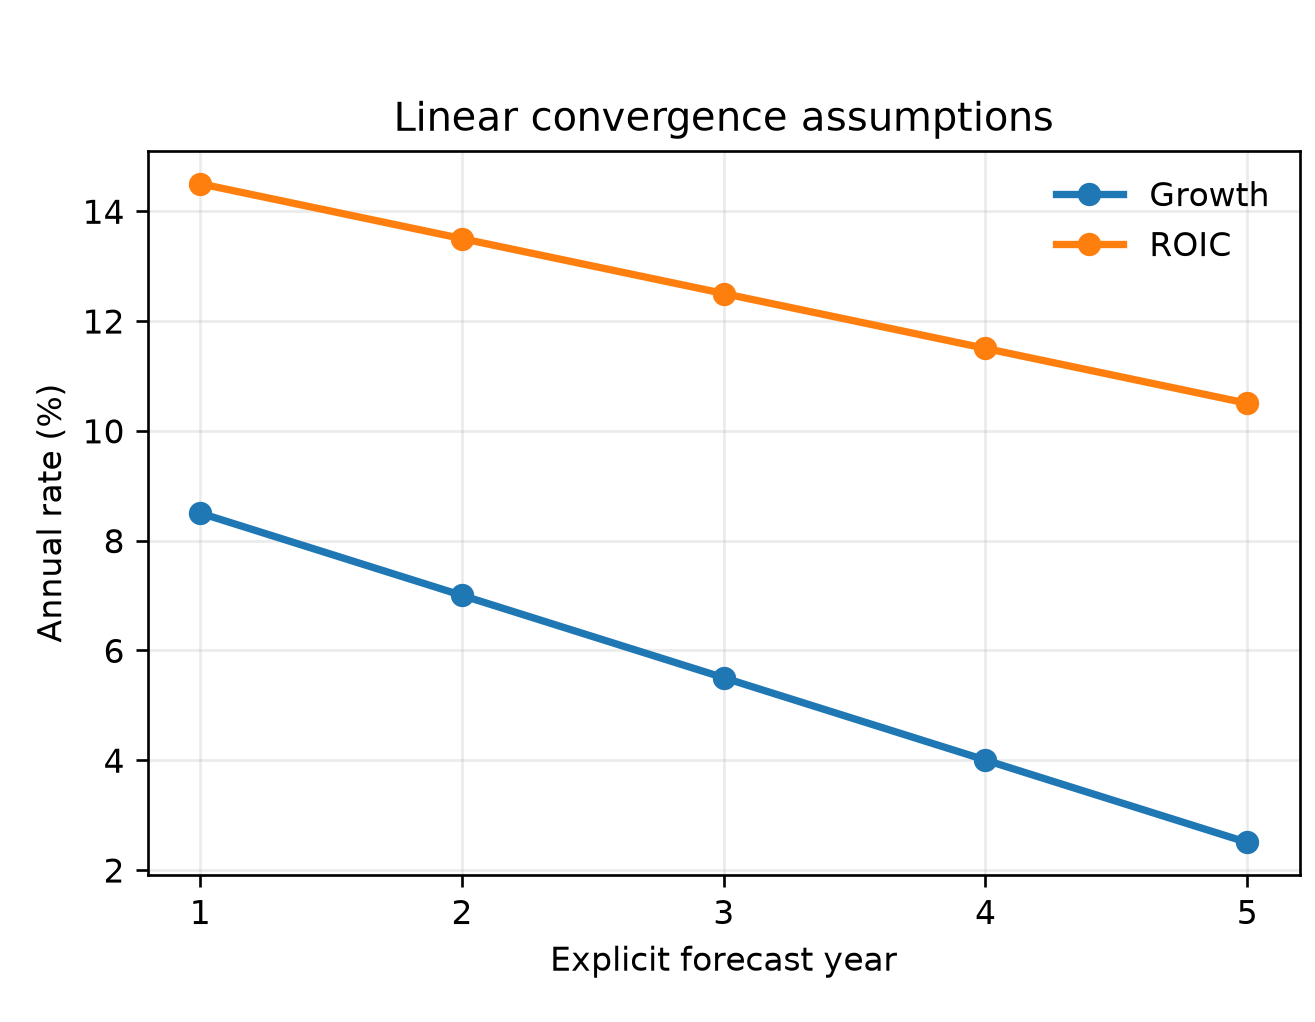
\includegraphics[width=0.90\linewidth]{figures/fig_dcf_growth_roic.png}
  \captionof{figure}{Common explicit-period DCF schedule: growth and ROIC converge linearly over the five-year horizon.}
  \label{fig:dcf_driver_schedule}
\par}
\end{minipage}\par

\noindent\begin{minipage}{\columnwidth}
{\centering
  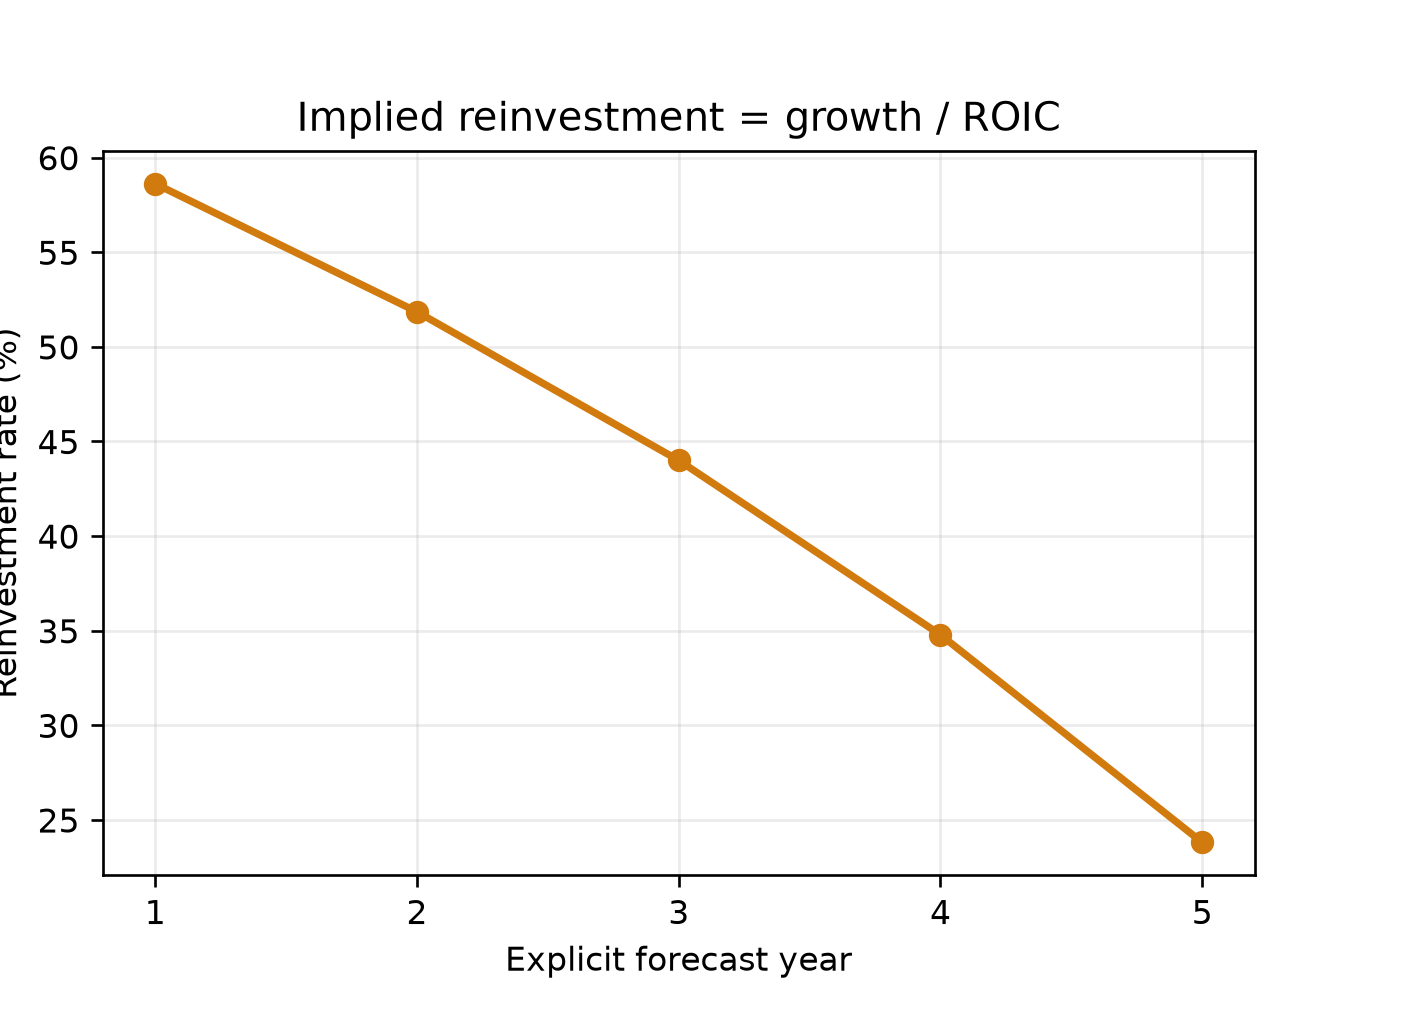
\includegraphics[width=0.90\linewidth]{figures/fig_dcf_reinvestment.png}
  \captionof*{figure}{\textbf{Figure~\ref{fig:dcf_driver_schedule} (continued).} The implied reinvestment rate, defined as growth divided by ROIC, falls from 58.62\% to 23.81\%.}
\par}
\end{minipage}\par

\subsection{Common stochastic WACC}
WACC follows the bounded mean-reverting process in Equation~(17), with inputs in Table~\ref{tab:dcf_inputs}. Its annual conditional standard deviation is 0.7308 percentage points. All branches reuse the same 8,192-path shock array; Figure~\ref{fig:wacc_assumptions} shows its distribution and zero-shock path.

\noindent\begin{minipage}{\columnwidth}
{\centering
  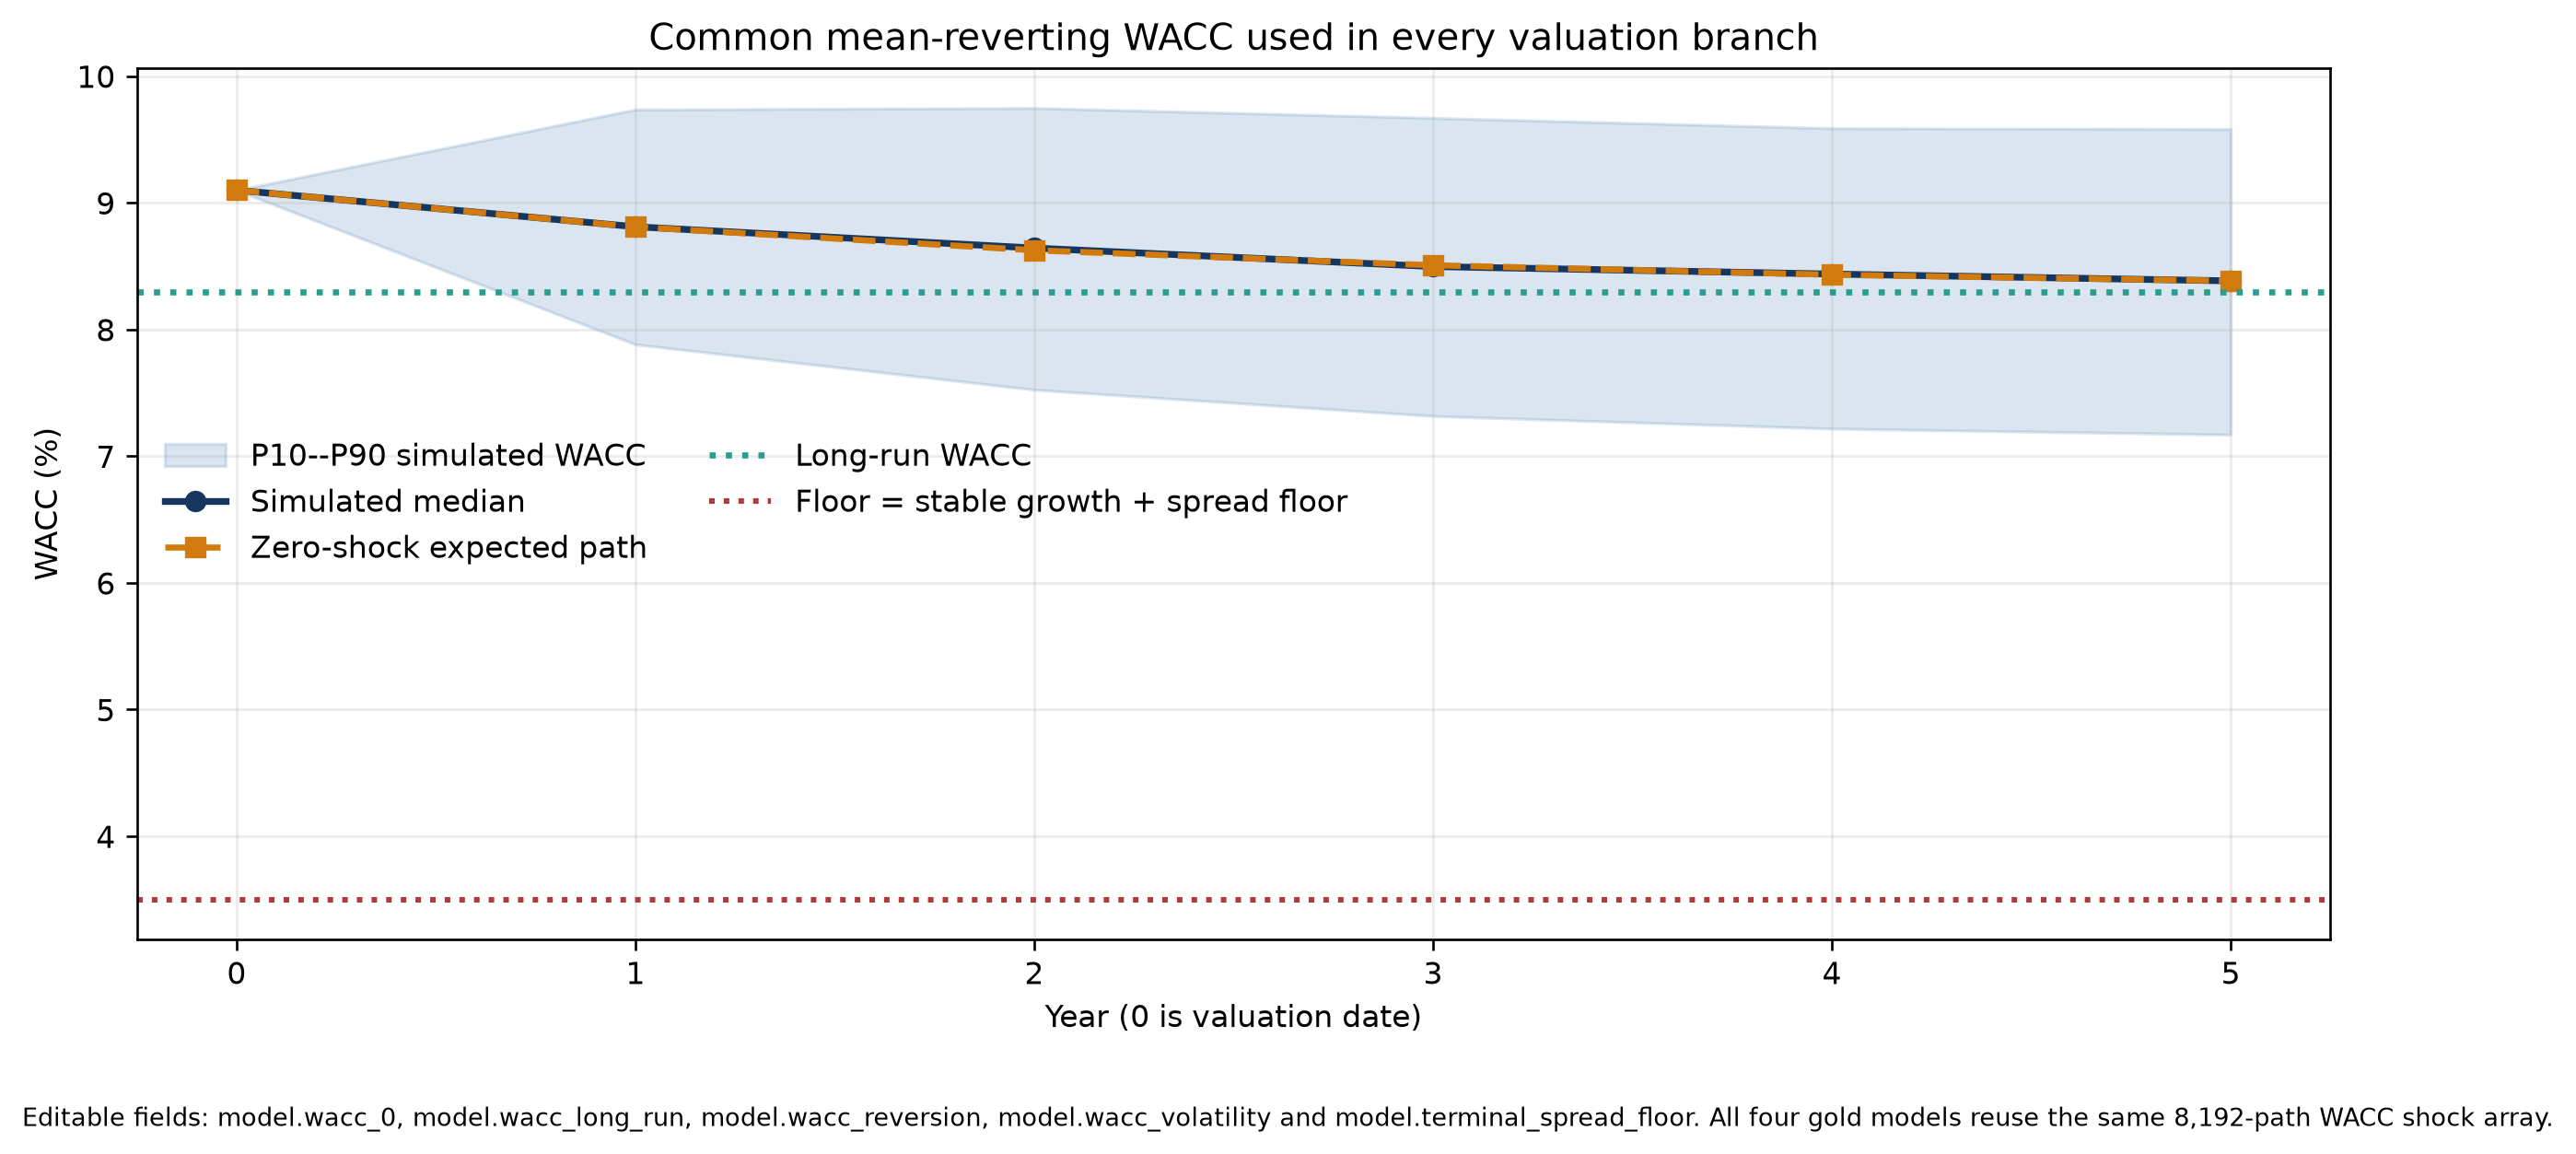
\includegraphics[width=0.95\columnwidth]{figures/fig_wacc_assumptions.png}
  \captionof{figure}{Common mean-reverting WACC. The band is the P10--P90 range from the shared 8,192-path shock array; the orange line is the zero-shock path and the dotted lines show the long-run level and admissibility floor.}
  \label{fig:wacc_assumptions}
\par}
\end{minipage}\par

\subsection{Terminal closure and sensitivity}
The terminal block uses $g_\infty=2.50\%$, $ROIC_\infty=10.50\%$ and terminal reinvestment of 23.81\%. At the current median terminal WACC of 8.384\%, the normalized terminal multiple is 13.27$\times$ final after-tax margin. The denominator is admitted only when $WACC_T>g_\infty$; the spread floor prevents a mechanically explosive closure in the simulated paths.

\noindent\begin{minipage}{\columnwidth}
{\centering
  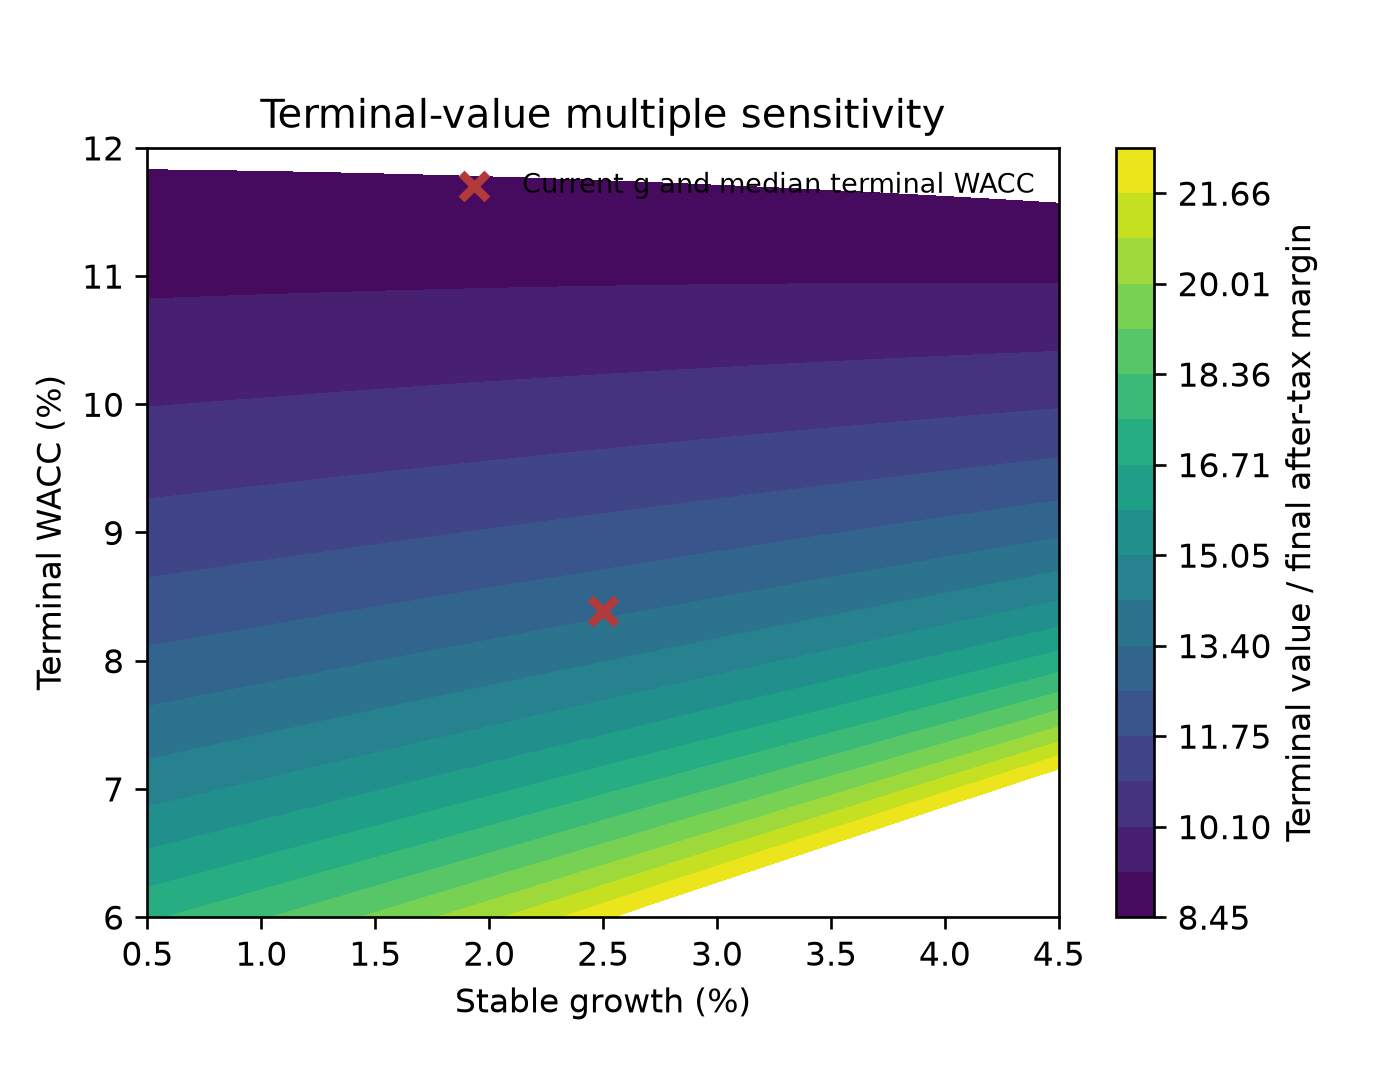
\includegraphics[width=0.90\linewidth]{figures/fig_terminal_multiple.png}
  \captionof{figure}{Terminal-value multiple sensitivity to stable growth and terminal WACC. The cross marks the configured stable-growth rate and current median terminal WACC.}
  \label{fig:terminal_value_mechanics}
\par}
\end{minipage}\par

\noindent\begin{minipage}{\columnwidth}
{\centering
  
\includegraphics[width=0.90\linewidth]{figures/fig_terminal_share.png}
  \captionof*{figure}{\textbf{Figure~\ref{fig:terminal_value_mechanics} (continued).} Present-value terminal share on positive-EV paths. Refreshed medians are 78.26\% for Black--Scholes, 78.31\% for Heston, 78.43\% for Bates and 78.27\% for Full Bates--Hawkes; bars show the P10--P90 range.}
\par}
\end{minipage}\par

\begin{table}[H]
\centering
\caption{Editable common DCF inputs.}
\label{tab:dcf_inputs}
\begin{tabularx}{\columnwidth}{@{}Xr@{}}
\toprule
Parameter & Value \\
\midrule
Tax rate & 25.00\% \\
$g_1\rightarrow g_\infty$ & 8.50--2.50\% \\
$ROIC_1\rightarrow ROIC_\infty$ & 14.50--10.50\% \\
$WACC_0\rightarrow\bar w$ & 9.10--8.30\% \\
WACC reversion & 0.45 \\
WACC volatility & 0.90\% \\
WACC floor/cap & 3.50/25.00\% \\
Terminal reinvestment & 23.81\% \\
\bottomrule
\end{tabularx}
\end{table}

\begin{methodbox}[Interpretation]
These are transparent methodological assumptions, not filing-calibrated Barrick estimates. Their materiality is visible: the terminal block supplies roughly three quarters of positive enterprise value. They should therefore be changed centrally and sensitivity-tested rather than hidden inside a single headline valuation.
\end{methodbox}
